\documentclass[11pt,letterpaper]{article}

\usepackage[T1]{fontenc}
\usepackage[margin=0.75in]{geometry}
\usepackage[table]{xcolor}
\usepackage{array}
\usepackage{tabularx}
\usepackage{enumitem}
\usepackage{fancyhdr}
\usepackage{graphicx}
\usepackage{hyperref}
\usepackage{listings}
\usepackage{tikz}
\usetikzlibrary{positioning}

\definecolor{LabBlue}{HTML}{0B5CAD}
\definecolor{LabTeal}{HTML}{00897B}
\definecolor{LabGreen}{HTML}{2E7D32}
\definecolor{LabOrange}{HTML}{EF6C00}
\definecolor{LabRed}{HTML}{C62828}
\definecolor{LabPurple}{HTML}{6A1B9A}
\definecolor{LabLightBlue}{HTML}{EAF4FF}
\definecolor{LabLightTeal}{HTML}{E6F7F5}
\definecolor{LabLightOrange}{HTML}{FFF3E0}
\definecolor{LabLightGreen}{HTML}{EAF7EA}
\definecolor{LabLightPurple}{HTML}{F4ECFA}

\hypersetup{
  colorlinks=true,
  linkcolor=LabBlue,
  urlcolor=LabTeal
}

\pagestyle{fancy}
\fancyhf{}
\lhead{\textcolor{LabBlue}{Lab 5 - Part 2: RoboLink}}
\rhead{\textcolor{LabTeal}{Mini Course Program 2026}}
\cfoot{\thepage}
\renewcommand{\headrulewidth}{0.6pt}

\setlength{\parindent}{0pt}
\setlength{\parskip}{6pt}
\setlength{\headheight}{14pt}
\setlist[itemize]{leftmargin=1.3em}
\setlist[enumerate]{leftmargin=1.5em}

\lstdefinestyle{ArduinoStyle}{
  basicstyle=\ttfamily\small,
  keywordstyle=\color{LabBlue}\bfseries,
  commentstyle=\color{LabGreen},
  stringstyle=\color{LabOrange},
  numbers=left,
  numberstyle=\tiny\color{gray},
  frame=single,
  rulecolor=\color{LabBlue},
  breaklines=true,
  tabsize=2
}

\newcommand{\colourbox}[3]{
  \vspace{0.2em}
  \noindent
  \fcolorbox{#1}{#2}{
    \begin{minipage}{0.96\linewidth}
      \vspace{0.45em}
      #3
      \vspace{0.45em}
    \end{minipage}
  }
  \vspace{0.4em}
}

\newcommand{\studentline}[1]{
  \vspace{0.2em}
  \textbf{#1}\enspace\hrulefill
}

\newcommand{\checkboxitem}[1]{
  \fbox{\rule{0pt}{1.15ex}\rule{1.15ex}{0pt}} \hspace{0.6em} #1
}

\begin{document}

\begin{center}
  
\includegraphics[width=0.42\linewidth]{assets/carleton_logo.png}
\end{center}

\begin{center}
  {\Huge \textbf{\textcolor{LabBlue}{Lab 5 - Part 2}}}\\[0.2em]
  {\Large \textbf{\textcolor{LabTeal}{RoboLink}}}\\[0.4em]
  {\large \textbf{Course:} RoboLink: Build and Drive Your Smartphone-Controlled Robot}\\[0.2em]
  {\large \textbf{Program:} Mini Course Program 2026, Carleton University}\\[0.2em]
  {\large \textbf{Instructors:} Dr. Mahmoud Sayed and Mahmoud Yassin}
\end{center}

\colourbox{LabBlue}{LabLightBlue}{
  \textbf{\textcolor{LabBlue}{Lab Mission}}\\
  In this lab, you will use the RoboLink Android app to drive a two-motor robot.
  The app sends wireless BLE commands to the Arduino Nano. The Arduino reads the
  command and controls the L9110 2-channel motor driver so the robot can move
  forward, move backward, turn left, turn right, and stop.
}

\studentline{Group Member Names}

\studentline{Date}

\section*{\textcolor{LabBlue}{1. Learning Goals}}

By the end of this lab, you should be able to:

\begin{itemize}
  \item Control a robot from an Android phone using BLE commands.
  \item Connect a BLE module and an L9110 motor driver to an Arduino Nano ATmega168.
  \item Explain how one command number becomes a robot movement.
  \item Use the Serial Monitor to debug wireless robot commands.
  \item Tune motor speed values so the robot drives more predictably.
  \item Troubleshoot common wiring, upload, connection, and movement problems.
\end{itemize}

\section*{\textcolor{LabBlue}{2. Big Idea}}

\colourbox{LabTeal}{LabLightTeal}{
  \textbf{\textcolor{LabTeal}{A robot command travels through a chain.}}\\
  The phone does not power the motors directly. It only sends a small command.
  The Arduino decides what the command means, and the motor driver supplies the
  motor current needed to move the robot.
}

\begin{center}
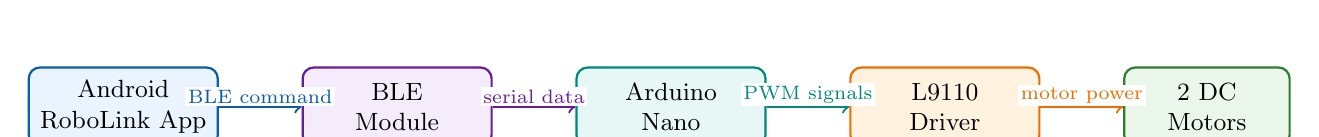
\begin{tikzpicture}[node distance=1.05cm, every node/.style={font=\small, align=center}]
  \node[draw=LabBlue, fill=LabLightBlue, rounded corners, thick, minimum width=2.4cm, minimum height=1.0cm] (phone) {Android\\RoboLink App};
  \node[draw=LabPurple, fill=LabLightPurple, rounded corners, thick, right=of phone, minimum width=2.4cm, minimum height=1.0cm] (ble) {BLE\\Module};
  \node[draw=LabTeal, fill=LabLightTeal, rounded corners, thick, right=of ble, minimum width=2.4cm, minimum height=1.0cm] (arduino) {Arduino\\Nano};
  \node[draw=LabOrange, fill=LabLightOrange, rounded corners, thick, right=of arduino, minimum width=2.4cm, minimum height=1.0cm] (driver) {L9110\\Driver};
  \node[draw=LabGreen, fill=LabLightGreen, rounded corners, thick, right=of driver, minimum width=2.1cm, minimum height=1.0cm] (motors) {2 DC\\Motors};
  \draw[->, thick, LabBlue] (phone) -- node[midway, above, fill=white, inner sep=1pt, font=\scriptsize]{BLE command} (ble);
  \draw[->, thick, LabPurple] (ble) -- node[midway, above, fill=white, inner sep=1pt, font=\scriptsize]{serial data} (arduino);
  \draw[->, thick, LabTeal] (arduino) -- node[midway, above, fill=white, inner sep=1pt, font=\scriptsize]{PWM signals} (driver);
  \draw[->, thick, LabOrange] (driver) -- node[midway, above, fill=white, inner sep=1pt, font=\scriptsize]{motor power} (motors);
\end{tikzpicture}
\end{center}

\section*{\textcolor{LabBlue}{3. Important Safety and Setup Notes}}

\colourbox{LabRed}{LabLightOrange}{
  \textbf{\textcolor{LabRed}{Keep the Wheels Off the Table First}}\\
  For the first test, lift the robot so the wheels can spin freely. This prevents
  the robot from driving off the table while you are checking the wiring and app
  connection.
}

\colourbox{LabOrange}{LabLightOrange}{
  \textbf{\textcolor{LabOrange}{Use Motor Power Correctly}}\\
  Do not power the motors only from the Arduino Nano 5V pin or USB. Use the motor
  battery or external motor power supply for the L9110 VCC pin. Connect Arduino
  GND, BLE module GND, L9110 GND, and battery GND together.
}

\colourbox{LabPurple}{LabLightPurple}{
  \textbf{\textcolor{LabPurple}{Special BLE Edition}}\\
  The module used in this lab looks like an HC-05 module, but it is a special
  edition that works with \textbf{BLE}, not classic Bluetooth SPP. Use the
  RoboLink Android app provided by your instructor.
}

\section*{\textcolor{LabBlue}{4. Materials}}

\begin{tabularx}{\linewidth}{>{\bfseries}p{0.34\linewidth}X}
Arduino Nano ATmega168 & Reads commands and controls the robot.\\
Special BLE HC-05-style module & Receives wireless commands from the Android app.\\
L9110 2-channel motor driver & Drives the left and right DC motors.\\
2 DC motors and robot chassis & Creates robot movement.\\
Android phone & Runs the RoboLink app. iPhone is not supported in this lab.\\
USB cable & Uploads code and opens the Serial Monitor.\\
Motor battery or external motor supply & Powers the motors through the L9110 driver.\\
Jumper wires and voltage divider resistors & Connect the modules safely.\\
\end{tabularx}

\section*{\textcolor{LabBlue}{5. Command Map}}

The RoboLink app sends one command number when a direction button is pressed.
When the button is released, the app sends \texttt{1} so the robot stops.

\begin{center}
\rowcolors{2}{LabLightTeal}{white}
\begin{tabular}{>{\centering\arraybackslash\bfseries}p{0.16\linewidth} p{0.46\linewidth} p{0.24\linewidth}}
\rowcolor{LabTeal}
\textcolor{white}{Command} & \textcolor{white}{Robot Action} & \textcolor{white}{When It Is Sent}\\
1 & Stop & Button released or Stop pressed\\
2 & Move forward & Forward pressed\\
3 & Move backward & Backward pressed\\
4 & Turn left & Left pressed\\
5 & Turn right & Right pressed\\
\end{tabular}
\end{center}

\section*{\textcolor{LabBlue}{6. Install and Prepare the Android App}}

\colourbox{LabRed}{LabLightOrange}{
  \textbf{\textcolor{LabRed}{Android Only}}\\
  The mobile app for this lab works on \textbf{Android phones only}. It is not
  designed for iPhone.
}

\colourbox{LabPurple}{LabLightPurple}{
  \textbf{\textcolor{LabPurple}{Before Scanning for the Robot}}\\
  Turn on \textbf{Bluetooth} and \textbf{Location/GPS}. Also give the RoboLink
  app all requested Android permissions for connectivity and location, such as
  Nearby Devices, Bluetooth, and Location permissions.
}

Install the app from this link:

\begin{center}
\url{https://drive.google.com/file/d/10tnT_rNqe7tGeGTrUGqdO2R689uXVynw/view?usp=drive_link}
\end{center}

\begin{center}
  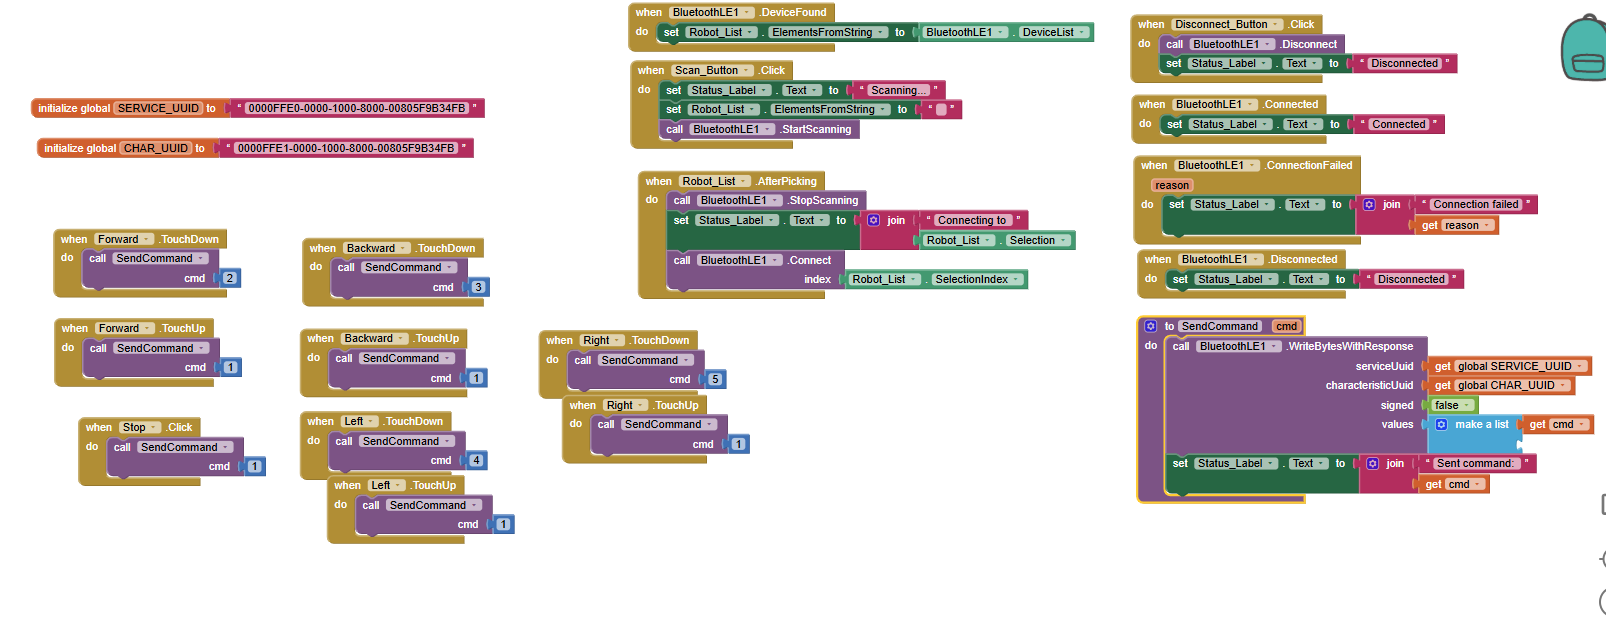
\includegraphics[width=0.95\linewidth]{assets/app_blocks.png}\\[-0.2em]
  {\small \textbf{MIT App Inventor blocks.} The app scans for a BLE module,
  connects to it, and sends command values when the robot buttons are used.}
\end{center}

\section*{\textcolor{LabBlue}{7. Wiring the BLE Module}}

\begin{center}
  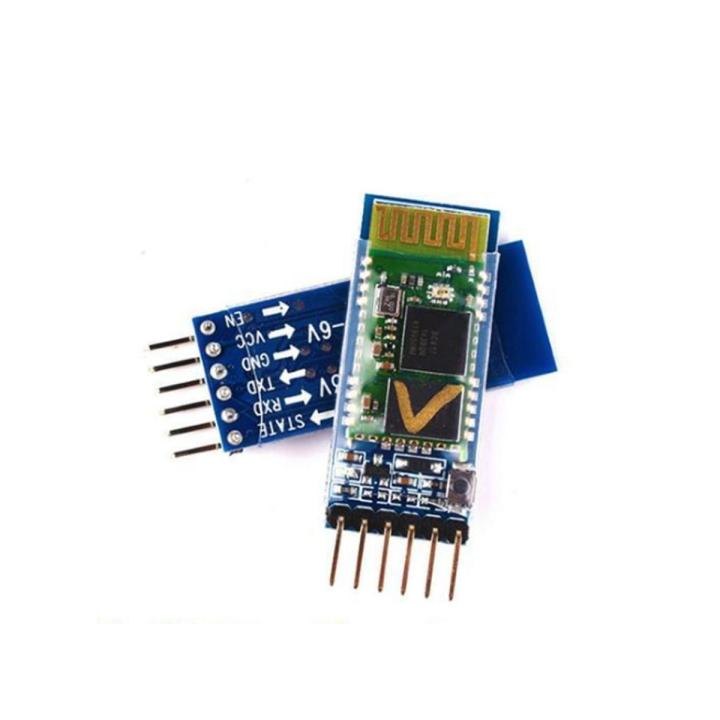
\includegraphics[width=0.34\linewidth]{assets/hc05_ble_module.jpg}\\[-0.2em]
  {\small \textbf{BLE module.} The module pins are labelled EN, VCC, GND, TXD,
  RXD, and STATE.}
\end{center}

\colourbox{LabRed}{LabLightOrange}{
  \textbf{\textcolor{LabRed}{Protect the Module RXD Pin}}\\
  Arduino D11 is a 5V signal. Many BLE module RXD pins expect about 3.3V. Use a
  voltage divider between Arduino D11 and module RXD.
}

\begin{center}
\rowcolors{2}{LabLightBlue}{white}
\begin{tabular}{>{\bfseries}c c p{0.42\linewidth}}
\rowcolor{LabBlue}
\textcolor{white}{BLE Module Pin} & \textcolor{white}{Arduino Nano Pin} & \textcolor{white}{Notes}\\
TXD & D10 & Module transmits to Arduino receive pin.\\
RXD & D11 & Use a voltage divider before RXD.\\
GND & GND & Must share ground with the Arduino and motor supply.\\
VCC & 5V or 3.3V & Use the correct power for your module board.\\
EN & Not used & Leave unconnected for this lab.\\
STATE & Not used & Leave unconnected for this lab.\\
\end{tabular}
\end{center}

\section*{\textcolor{LabBlue}{8. Wiring the L9110 Motor Driver}}

\begin{center}
  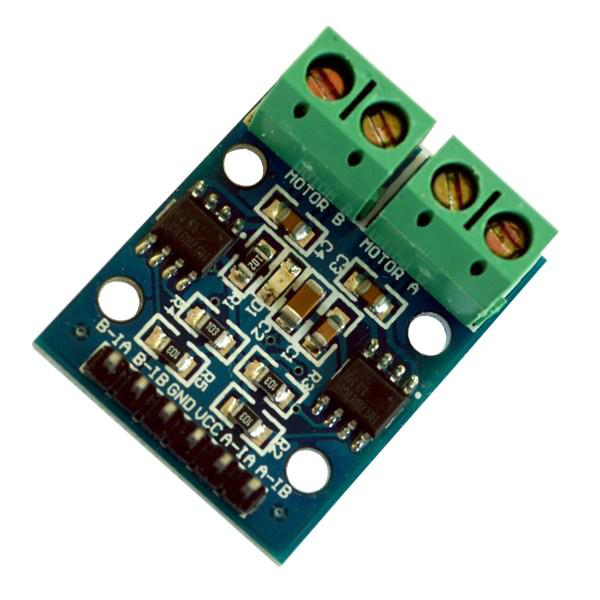
\includegraphics[width=0.40\linewidth]{assets/l9110_driver.png}\\[-0.2em]
  {\small \textbf{L9110 2-channel motor driver.} The green screw terminals
  connect to Motor A and Motor B.}
\end{center}

\begin{center}
\rowcolors{2}{LabLightBlue}{white}
\begin{tabular}{>{\bfseries}c c p{0.38\linewidth}}
\rowcolor{LabBlue}
\textcolor{white}{L9110 Pin} & \textcolor{white}{Arduino Nano Pin} & \textcolor{white}{Purpose}\\
A-IA & D3 & Left motor forward PWM signal.\\
A-IB & D5 & Left motor backward PWM signal.\\
B-IA & D6 & Right motor forward PWM signal.\\
B-IB & D9 & Right motor backward PWM signal.\\
GND & GND & Connect to Arduino GND and battery GND.\\
VCC & Motor power & External motor power, usually 2.5V to 12V.\\
\end{tabular}
\end{center}

\colourbox{LabPurple}{LabLightPurple}{
  \textbf{\textcolor{LabPurple}{Before Powering the Motors}}\\
  Ask your teacher to check the BLE wiring, L9110 wiring, battery polarity, and
  shared ground before turning on motor power.
}

\section*{\textcolor{LabBlue}{9. Arduino IDE Setup}}

\begin{enumerate}
  \item Open the Arduino IDE or PlatformIO project.
  \item Open the Lab 5 Part 2 RoboLink code.
  \item Select \textbf{Tools \(\rightarrow\) Board \(\rightarrow\) Arduino AVR Boards \(\rightarrow\) Arduino Nano}.
  \item Select \textbf{Tools \(\rightarrow\) Processor \(\rightarrow\) ATmega168}.
  \item Select the correct \textbf{Tools \(\rightarrow\) Port}.
  \item Upload the code.
  \item Open \textbf{Tools \(\rightarrow\) Serial Monitor}.
  \item Set the baud rate to \textbf{9600}.
\end{enumerate}

\section*{\textcolor{LabBlue}{10. Experiment Procedure}}

\subsection*{\textcolor{LabTeal}{Part A: USB Test First}}

Before using the app, test the code from the Serial Monitor.

\begin{enumerate}
  \item Keep the robot wheels lifted off the table.
  \item Open the Serial Monitor at 9600 baud.
  \item Send \texttt{1}, \texttt{2}, \texttt{3}, \texttt{4}, and \texttt{5}.
  \item Watch the wheels and read the printed messages.
\end{enumerate}

\begin{center}
\rowcolors{2}{LabLightBlue}{white}
\begin{tabularx}{\linewidth}{>{\bfseries}c X X}
\rowcolor{LabBlue}
\textcolor{white}{Command} & \textcolor{white}{Expected Movement} & \textcolor{white}{What Actually Happened?}\\
1 & Stop & \\
2 & Forward & \\
3 & Backward & \\
4 & Turn left slowly & \\
5 & Turn right slowly & \\
\end{tabularx}
\end{center}

\subsection*{\textcolor{LabTeal}{Part B: Connect the RoboLink App}}

\begin{enumerate}
  \item Turn on Bluetooth and Location/GPS on the Android phone.
  \item Check that the app permissions are allowed.
  \item Open the RoboLink app.
  \item Scan for the BLE module.
  \item Select the robot BLE module and wait for connection.
  \item Keep the Serial Monitor open so you can see the commands arriving.
\end{enumerate}

\colourbox{LabPurple}{LabLightPurple}{
  \textbf{Connection observation:} What name appeared for your BLE module?\\[1.5em]
  \hrulefill
}

\subsection*{\textcolor{LabTeal}{Part C: Drive the Robot from the App}}

\begin{enumerate}
  \item Press and hold Forward. Release the button and check that the robot stops.
  \item Press and hold Backward. Release the button and check that the robot stops.
  \item Press and hold Left. Release the button and check that the robot stops.
  \item Press and hold Right. Release the button and check that the robot stops.
  \item If the robot moves safely while lifted, place it on the floor and test again.
\end{enumerate}

\colourbox{LabGreen}{LabLightGreen}{
  \textbf{Observation:} Did the robot stop when you released each app button?\\[1.5em]
  \hrulefill
}

\subsection*{\textcolor{LabTeal}{Part D: Tune the Movement}}

The code has three important speed values:

\begin{lstlisting}[style=ArduinoStyle]
const int LEFT_MOTOR_SPEED = 200;
const int RIGHT_MOTOR_SPEED = 200;
const int TURN_SPEED = 140;
\end{lstlisting}

\begin{itemize}
  \item If the robot curves left while going forward, the left motor may be slower.
  \item If the robot curves right while going forward, the right motor may be slower.
  \item If turning is too weak, increase \texttt{TURN\_SPEED} a little.
  \item If turning is too fast, decrease \texttt{TURN\_SPEED} a little.
\end{itemize}

\colourbox{LabGreen}{LabLightGreen}{
  \textbf{Your tuning notes:}\\[1.5em]
  \hrulefill\\[1.5em]
  \hrulefill
}

\subsection*{\textcolor{LabTeal}{Part E: Mini Driving Challenge}}

Use the app to drive your robot through a simple path chosen by your teacher.
Drive slowly and stop if the robot leaves the course.

\colourbox{LabPurple}{LabLightPurple}{
  \textbf{What strategy helped you control the robot smoothly?}\\[2em]
  \hrulefill\\[1.5em]
  \hrulefill
}

\section*{\textcolor{LabBlue}{11. What Is Happening in the Code?}}

\begin{tabularx}{\linewidth}{>{\bfseries}p{0.28\linewidth}X}
\texttt{SoftwareSerial BT(10, 11)} & Creates a serial connection to the BLE module using Arduino pins D10 and D11.\\
\texttt{BT.available()} & Checks whether the phone app sent a command.\\
\texttt{BT.read()} & Reads one command byte from the BLE module.\\
\texttt{normalizeCommand()} & Allows both app commands and Serial Monitor test commands to work.\\
\texttt{handleCommand()} & Chooses stop, forward, backward, left, or right.\\
\texttt{analogWrite()} & Sends PWM values to control motor speed.\\
\texttt{stopMotors()} & Sets all four L9110 input pins LOW so the robot stops.\\
\texttt{moveTo()} & Adds a short pause when changing direction.\\
\end{tabularx}

\colourbox{LabOrange}{LabLightOrange}{
  \textbf{\textcolor{LabOrange}{Why are some motor pins LOW?}}\\
  Each L9110 motor channel uses two input pins. To spin one direction, one pin
  receives PWM and the other pin is LOW. To spin the opposite direction, the
  pins switch roles. When stopping, all four driver input pins are set LOW.
}

\section*{\textcolor{LabBlue}{12. Expected Problems and Fixes}}

\begin{center}
\rowcolors{2}{LabLightOrange}{white}
\begin{tabularx}{\linewidth}{>{\bfseries}p{0.24\linewidth}X X}
\rowcolor{LabOrange}
\textcolor{white}{Problem} & \textcolor{white}{Possible Cause} & \textcolor{white}{What To Try}\\
Upload fails & Wrong board, processor, or port & Select Arduino Nano, ATmega168, and the correct port.\\
App cannot find module & Bluetooth off, Location/GPS off, permissions missing, or BLE module not powered & Turn on Bluetooth and Location/GPS, allow app permissions, and check module power.\\
Serial Monitor shows no app commands & TXD/RXD wiring problem or wrong baud rate & Set Serial Monitor to 9600. Check TXD to D10 and D11 to RXD through the voltage divider.\\
Nothing moves & Motor battery missing, shared ground missing, or L9110 wiring error & Check motor power, GND connections, D3, D5, D6, and D9.\\
Robot moves when button is released & Stop command is not arriving or app connection dropped & Check Serial Monitor for command 1 and reconnect the app.\\
Robot drives backward on Forward & Motor wires are reversed & Swap the two wires on the motor terminals or adjust the movement function.\\
Left and right are reversed & Motor A and Motor B are swapped, or one motor is reversed & Check which motor is connected to Motor A and Motor B.\\
One motor is slower & DC motors are not perfectly matched & Tune \texttt{LEFT\_MOTOR\_SPEED} and \texttt{RIGHT\_MOTOR\_SPEED}.\\
Turns are too fast or too slow & \texttt{TURN\_SPEED} needs tuning & Adjust \texttt{TURN\_SPEED} in small steps.\\
Robot resets when motors start & Motor supply cannot provide enough current & Use a stronger motor battery or reduce speed.\\
\end{tabularx}
\end{center}

\section*{\textcolor{LabBlue}{13. Reflection Questions}}

Answer in full sentences.

\begin{enumerate}
  \item Why does the app send a stop command when you release a direction button?
  \vspace{2em}

  \item Why should we test the robot with the wheels lifted before driving it on the floor?
  \vspace{2em}

  \item What is the job of the Arduino in this robot system?
  \vspace{2em}

  \item What is the job of the L9110 motor driver?
  \vspace{2em}

  \item Why do the Arduino, BLE module, L9110 driver, and motor battery need a shared GND?
  \vspace{2em}

  \item If the robot does not drive straight, what evidence would help you decide which motor speed to change?
  \vspace{2em}

  \item What is one improvement you would make to the RoboLink robot or app?
  \vspace{2em}
\end{enumerate}

\section*{\textcolor{LabBlue}{14. Exit Ticket}}

\colourbox{LabBlue}{LabLightBlue}{
  \textbf{In one or two sentences:} Explain how pressing a button on a phone can make a robot move.\\[3em]
  \hrulefill\\[1.5em]
  \hrulefill
}

\section*{\textcolor{LabBlue}{15. Teacher Check}}

\colourbox{LabTeal}{LabLightTeal}{
  \textbf{\textcolor{LabTeal}{Teacher Checklist}}\\[0.4em]
  \begin{tabularx}{\linewidth}{>{\bfseries}p{0.58\linewidth}X}
    \checkboxitem{BLE module wiring checked} & Notes: \hrulefill\\[1.0em]
    \checkboxitem{L9110 motor wiring checked} & Notes: \hrulefill\\[1.0em]
    \checkboxitem{Code uploaded} & Notes: \hrulefill\\[1.0em]
    \checkboxitem{Android app connected to BLE module} & Notes: \hrulefill\\[1.0em]
    \checkboxitem{Robot responds to app commands} & Notes: \hrulefill\\[1.0em]
    \checkboxitem{Robot stops when app button is released} & Notes: \hrulefill\\[1.0em]
    \checkboxitem{Students completed observations} & Notes: \hrulefill\\[1.0em]
    \checkboxitem{Students answered reflection questions} & Notes: \hrulefill\\
  \end{tabularx}
}

\end{document}
